\documentclass[main]{subfiles}

\begin{document}

\begin{figure}[h]
    \centering
    %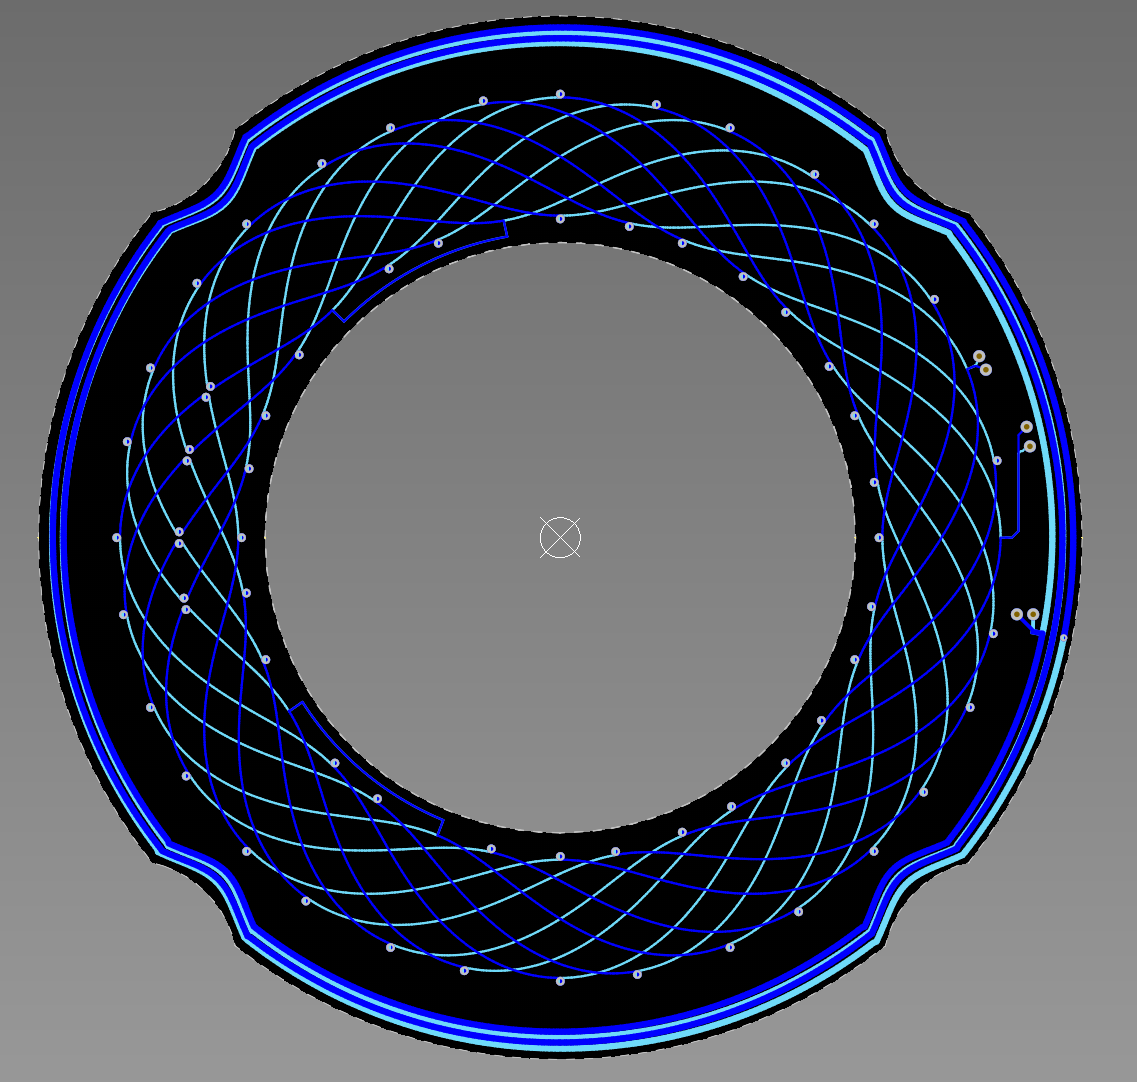
\includegraphics[width=0.6\linewidth]{img/pcb_coil_bucaneve.png}
    \caption{Pcb Coils}
    \label{FIG_SENSOR_PCB_COILS}
\end{figure}

The coils have been realized on the lower internal layer and the bottom layer of
the \ac{PCB}, using blind vias to avoid interference with top layer components.
In this way, the distance between the 2 layers forming the coils is minimized
and the one between coil and logic is maximized.
A $2.8 mm$ board has been used to keep the logic circuit and the coils even more 
spaced.

In figure \ref{FIG_SENSOR_PCB_COILS} you can see that the TX Coil is made with a
thicker trace ($0.45 mm$), in order to reduce the parasitic resistance, and it
has 4 turns.
The RX Coils are instead made with regular trace width ($0.2 mm$), since they 
don't need to carry any current.
To amplify the received signal, the RX coil has been realized with 2 turns 
connected in series.

The second turn of the RX coils has been realized with an angular displacement
of

\begin{equation}
    \Phi_{mecc} = 10^\circ
\end{equation}

which gives an electrical angle of 

\begin{equation}
    \Phi_{el} = PP \cdot \Phi_{mecc} = 40^\circ
\end{equation}

Due to this displacement the sinewave amplitude will not simply be doubled, but 
the 2 vectors will add with a vector sum (figure \ref{}).

\begin{figure}[h]
    \centering
    %\includegraphics[width=0.5/linewidth]{}
    \caption{Vector sum of 2 coils voltages}
\end{figure}

\end{document}